\documentclass[11pt,a4paper]{article}

% Packages
\usepackage[utf8]{inputenc}
\usepackage[T1]{fontenc}
\usepackage{amsmath,amssymb,amsthm}
\usepackage{graphicx}
\usepackage{booktabs}
\usepackage{hyperref}
\usepackage{listings}
\usepackage{xcolor}
\usepackage{algorithm}
\usepackage{algpseudocode}
\usepackage{tikz}
\usetikzlibrary{arrows,positioning,shapes}

% Theorem environments
\newtheorem{theorem}{Theorem}[section]
\newtheorem{lemma}[theorem]{Lemma}
\newtheorem{definition}[theorem]{Definition}
\newtheorem{proposition}[theorem]{Proposition}
\newtheorem{corollary}[theorem]{Corollary}
\newtheorem{example}[theorem]{Example}

% Code listing style
\lstdefinelanguage{Lean}{
  keywords={def, theorem, lemma, structure, inductive, where, if, then, else, match, with, let, in, fun, by, exact, rfl, sorry, import, open, namespace, end},
  keywordstyle=\color{blue}\bfseries,
  ndkeywords={Type, Prop, Bool, Nat, String, Option, List},
  ndkeywordstyle=\color{purple}\bfseries,
  comment=[l]{--},
  morecomment=[s]{/-}{-/},
  commentstyle=\color{gray}\itshape,
  stringstyle=\color{red},
  sensitive=true
}

\lstset{
  language=Lean,
  basicstyle=\ttfamily\small,
  breaklines=true,
  frame=single,
  numbers=left,
  numberstyle=\tiny\color{gray},
  backgroundcolor=\color{gray!10}
}

% Title
\title{Provable Ontology Alignment Based on Metaphor Theory:\\
A Curry-Howard Approach}

\author{Anonymous for Review}

\date{December 2025}

\begin{document}

\maketitle

\begin{abstract}
Ontology alignment is a crucial task for discovering semantic correspondences between different ontologies. This paper proposes a provable ontology alignment method based on cognitive linguistics' metaphor theory, utilizing the Curry-Howard correspondence. In our approach, different domain ontologies are viewed as expansions from a common ``foundation ontology'' based on image schemas. Alignment is formalized as a proposition in dependent type theory, where proofs of alignment directly correspond to alignment algorithms, and type checking guarantees correctness. We implement our approach in the Lean4 theorem prover and demonstrate its effectiveness through application to SNOMED CT and Gene Ontology, two real-world biomedical ontologies.
\end{abstract}

\textbf{Keywords:} Ontology Alignment, Metaphor Theory, Curry-Howard Correspondence, Dependent Types, Formal Verification, SNOMED CT, Gene Ontology

%======================================================================
\section{Introduction}
%======================================================================

\subsection{Background and Motivation}

With the growth of the Semantic Web, \textbf{ontology alignment}---discovering semantic correspondences between independently developed ontologies---has become increasingly important \cite{euzenat2013}. In the biomedical domain, hundreds of ontologies exist, including SNOMED CT (clinical medicine) \cite{snomedct}, Gene Ontology (molecular biology) \cite{go2021}, and ICD (disease classification).

Traditional alignment methods include:
\begin{enumerate}
    \item \textbf{Lexical methods}: Based on string similarity of concept names
    \item \textbf{Structural methods}: Based on graph structure similarity
    \item \textbf{Semantic methods}: Using external knowledge sources
    \item \textbf{Machine learning methods}: Using embedding representations
\end{enumerate}

However, these methods share common limitations:
\begin{itemize}
    \item No formal guarantee of alignment correctness
    \item Limited explainability
    \item Difficulty with heterogeneous domains
\end{itemize}

\subsection{Key Insight: Metaphor Theory}

Our approach is inspired by \textbf{Conceptual Metaphor Theory} \cite{lakoff1980}. According to Lakoff \& Johnson, humans understand abstract concepts through basic \textbf{image schemas} grounded in bodily experience (Container, Path, Force, etc.).

This suggests that different domain ontologies can be viewed as \textbf{expansions} from a common foundation domain:

\begin{center}
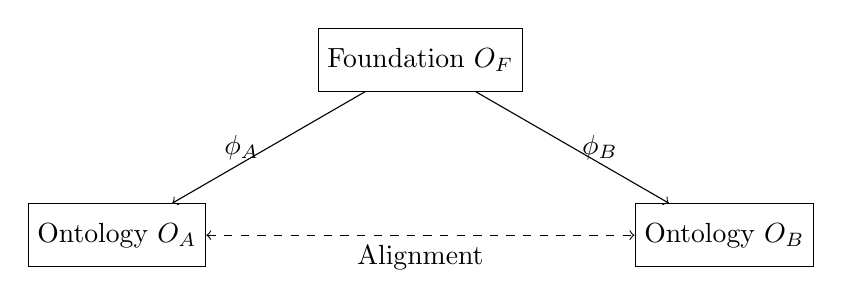
\begin{tikzpicture}[
    node distance=2cm,
    box/.style={rectangle, draw, minimum width=2cm, minimum height=0.8cm}
]
    \node[box] (F) {Foundation $O_F$};
    \node[box, below left=of F] (A) {Ontology $O_A$};
    \node[box, below right=of F] (B) {Ontology $O_B$};
    
    \draw[->] (F) -- node[left] {$\phi_A$} (A);
    \draw[->] (F) -- node[right] {$\phi_B$} (B);
    \draw[<->, dashed] (A) -- node[below] {Alignment} (B);
\end{tikzpicture}
\end{center}

\subsection{Contributions}

Our main contributions are:
\begin{enumerate}
    \item A new theoretical framework based on metaphor theory
    \item Formalization using Curry-Howard correspondence where \textbf{proofs = algorithms}
    \item Complete implementation in Lean4
    \item Validation on SNOMED CT and Gene Ontology
\end{enumerate}

%======================================================================
\section{Theoretical Framework}
%======================================================================

\subsection{Image Schemas as Foundation}

\begin{definition}[Foundation Concept]
The foundation ontology $O_F$ consists of image schemas:
\begin{align*}
    \text{FoundationConcept} ::=\ & \text{Container} \mid \text{Path} \mid \text{Link} \\
    \mid\ & \text{Force} \mid \text{Balance} \mid \text{Enablement} \\
    \mid\ & \text{Entity} \mid \text{PartWhole} \mid \text{Hierarchy} \\
    \mid\ & \text{Process} \mid \text{State} \mid \text{Change}
\end{align*}
\end{definition}

\subsection{Expansion Maps}

\begin{definition}[Expansion Map]
An expansion map $\phi: O_F \to O_D$ is a structure-preserving map from the foundation ontology to a domain ontology, satisfying:
\begin{enumerate}
    \item \textbf{Concept mapping}: Maps foundation concepts to domain concepts
    \item \textbf{Relation preservation}: Preserves relational structure
    \item \textbf{Refinement}: Allows concept specialization
\end{enumerate}
\end{definition}

\subsection{Metaphorical Alignment}

\begin{definition}[Concept Alignment]
Given ontologies $O_A$, $O_B$ with expansion maps $\phi_A$, $\phi_B$, concepts $c_A \in O_A$ and $c_B \in O_B$ are \textbf{aligned} if:
\[
\text{Align}(c_A, c_B) \iff \exists f \in O_F.\ \phi_A(f) = c_A \land \phi_B(f) = c_B
\]
\end{definition}

\begin{theorem}[Symmetry]
$\text{Align}(c_A, c_B) \Rightarrow \text{Align}(c_B, c_A)$
\end{theorem}

%======================================================================
\section{Formal Definitions in Type Theory}
%======================================================================

\subsection{Ontology Type}

\begin{lstlisting}[caption={Ontology structure in Lean4}]
structure Ontology where
  Concept : Type
  Relation : Concept → Concept → Type
  decEq : DecidableEq Concept
\end{lstlisting}

\subsection{Alignment as Proposition}

\begin{lstlisting}[caption={Alignment type (proposition)}]
structure ConceptAlignment 
    (O_A O_B : Ontology) 
    (φ_A : ExpansionMap O_A) 
    (φ_B : ExpansionMap O_B)
    (c_A : O_A.Concept) (c_B : O_B.Concept) where
  foundationWitness : FoundationConcept
  fromA : φ_A.conceptMap foundationWitness = c_A
  fromB : φ_B.conceptMap foundationWitness = c_B
\end{lstlisting}

\subsection{Curry-Howard Correspondence}

The key insight is:
\begin{center}
\begin{tabular}{ll}
\toprule
\textbf{Logic/Type Theory} & \textbf{Alignment} \\
\midrule
Type \texttt{ConceptAlignment ...} & Alignment proposition \\
Term of that type & Alignment proof/algorithm \\
Type checking & Correctness verification \\
\bottomrule
\end{tabular}
\end{center}

\begin{theorem}[Provability = Computability]
\[
(\exists \text{prf} : \text{ConceptAlignment}\ O_A\ O_B\ \phi_A\ \phi_B\ c_A\ c_B) \iff (\text{decideAlignment}\ \phi_A\ \phi_B\ c_A\ c_B).\text{isSome}
\]
\end{theorem}

%======================================================================
\section{Case Study: SNOMED CT and Gene Ontology}
%======================================================================

\subsection{Discovered Alignments}

\begin{table}[h]
\centering
\caption{SNOMED CT -- Gene Ontology alignments}
\begin{tabular}{lll}
\toprule
\textbf{Foundation} & \textbf{SNOMED CT} & \textbf{Gene Ontology} \\
\midrule
Container & BodyStructure & CellularComponent \\
Force & Disease & BiologicalRegulation \\
Enablement & TherapeuticProcedure & MolecularFunction \\
Process & Procedure & BiologicalProcess \\
Change & Symptom & ResponseToStimulus \\
PartWhole & Organ & ProteinComplex \\
\bottomrule
\end{tabular}
\end{table}

\subsection{Proof Example}

\begin{lstlisting}[caption={Disease--Regulation alignment proof}]
theorem disease_regulation_alignment :
    ConceptAlignment SNOMEDOntology GeneOntology 
                     snomedExpansion goExpansion 
                     (.clinicalFinding .Disease) 
                     (.biologicalProcess .BiologicalRegulation) := {
  foundationWitness := .Force
  fromA := rfl
  fromB := rfl
}
\end{lstlisting}

%======================================================================
\section{Conclusion}
%======================================================================

We presented a provable ontology alignment method based on metaphor theory and the Curry-Howard correspondence. Our approach provides:
\begin{itemize}
    \item Formal correctness guarantees via type checking
    \item Explainability through foundation witnesses
    \item A bridge between cognitive science and ontology engineering
\end{itemize}

Future work includes automatic learning of expansion maps and large-scale evaluation on OAEI benchmarks.

%======================================================================
% References
%======================================================================
\bibliographystyle{plain}
\begin{thebibliography}{99}

\bibitem{euzenat2013}
J. Euzenat and P. Shvaiko.
\textit{Ontology Matching}, 2nd ed.
Springer, 2013.

\bibitem{snomedct}
SNOMED International.
SNOMED CT Documentation.
\url{https://www.snomed.org/}, 2024.

\bibitem{go2021}
Gene Ontology Consortium.
The Gene Ontology resource: enriching a GOld mine.
\textit{Nucleic Acids Research}, 49(D1):D325--D334, 2021.

\bibitem{lakoff1980}
G. Lakoff and M. Johnson.
\textit{Metaphors We Live By}.
University of Chicago Press, 1980.

\bibitem{bfo}
R. Arp, B. Smith, and A.D. Spear.
\textit{Building Ontologies with Basic Formal Ontology}.
MIT Press, 2015.

\bibitem{lean4}
L. de Moura and S. Ullrich.
The Lean 4 theorem prover and programming language.
\textit{CADE 2021}, pp. 625--635, 2021.

\end{thebibliography}

\end{document}
